\chapter{Introduktion} \label{sec:intro}
Future Cropping er et forsknings projekt, oprettet af Miljøstyrelsen, der i samarbejde med Datalogisk institut og institut for Plante- og Miljøvidenskab, har til formål at automatisere detektionen af ukrudt i marker. I dag bekæmpes ukrudt, ved at sprøjte hele marken med pesticider, uvidende om, hvor ukrudtet er placeret. Projektet har til formål at nedsætte forbruget af pesticider, ved hjælp af en drone\footnote{UAV (eng. unmanned aerial vehicle} udstyret med et kamera. Dronen tager et antal overlappende luftbilleder af en mark, disse billeder analyseres af en algoritme, der identificere, hvor ukrudtet befinder sig i de enkelte billeder. Resultatet af denne analyse overføres til et globalt koordinatsystem af hele marken, hvilket kan opnås ved at bestemme de geometriske relationer imellem billederne. Det samlede ukrudtskort, vil angive ukrudtets placering og derved, hvor der er behov for pesticider \cite{drone}.
\begin{figure}[H]
    \centering
    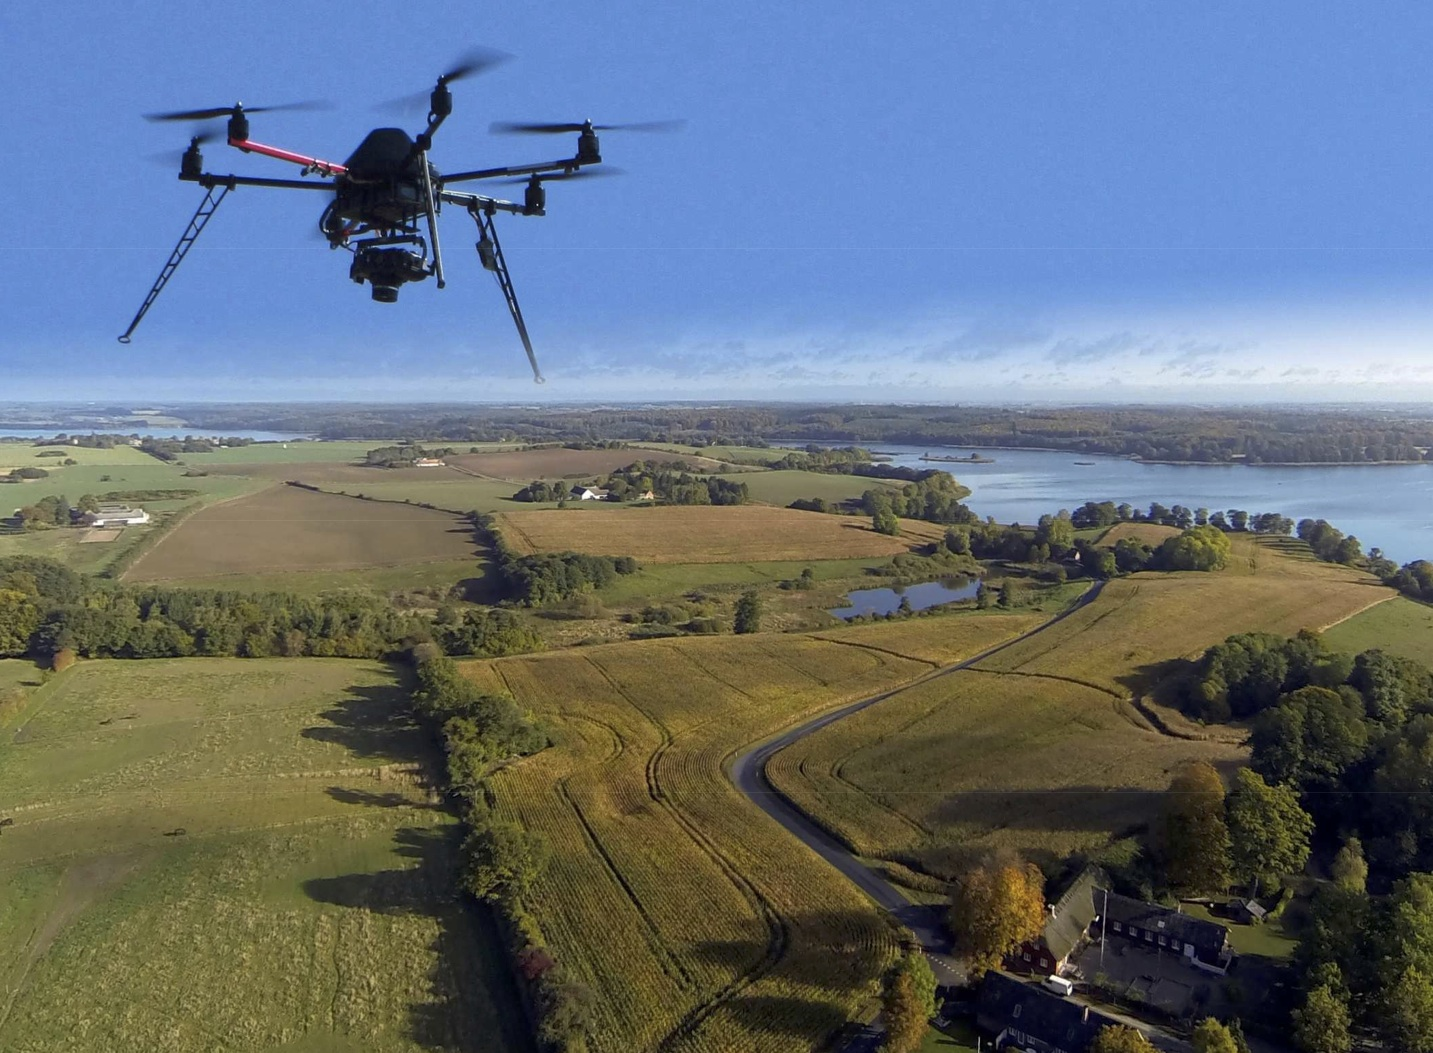
\includegraphics[width=0.45\textwidth]{fig/drone4.jpg}
     \vspace{-0.5em}
    \begin{center}    
       \caption{\textcolor{gray}{\footnotesize \textit{ }}}
    \label{fig:difference}
     \end{center}
     \vspace{-3em}
  \end{figure} \noindent
\section{Opgavens problemfelt} \label{subsec:felt}
Opgavens afsæt i dette projekt er bestemmelsen af, hvordan de individuelle billeder af marken passer sammen, hvilket er det første skridt i etableringen af ukrudtskortet. De geometriske relationer bestemmes, ved at etablere korrespondancer imellem billederne. Denne teknik hedder korrespondanceanalyse, og går ud på at determinere, for to eller flere billeder, hvilke punkter der korrespondere på tværs af billederne. Korrespondanceanalysen imellem to billeder, består af følgende trin: 
\begin{enumerate}
\item{Interessante punkter udvælges i begge billeder, som resultat af at anvende en række matematiske modeller på billederne. Formålet ved dette stadie er udvælge de samme punkter, hvor billederne overlapper, hvilket er muligt da markbillederne i gennemsnit overlapper hinanden med ca. 70 \%.}
\item{En deskriptor beskriver, for hvert interessepunkt den lokale billedstruktur omkring punktet.}
\item{Hver beskrivelse af punkter sammenlignes med beskrivelser af punkter i det andet billede  for at undersøge om punkterne korrespondere.}
\end{enumerate}
\section{Rapportens Opbygning}
\section{Problemformulering} \label{subsec:form}
Med udgangspunkt i litteraturen indenfor
korrespondanceanalyse samt implementering af
flere eksisterende metoder er spørgsmålet, hvilke metoder, der teoretisk og praktisk, bedst anvendes til korrespondanceanalyse af markbilleder \\ \\
\section{Udvidelse af problemformuleringen}
Der opstilles en beskrivelse af forskellige udvalgte metoder, der indgår i korrespondanceanalysens pipeline og foretages korrespondanceanalyse af markbillederne, ved implementering af disse metoder. \\
Det eksperimentelle fokus i opgaven vil ligge på afprøvning, af de implementerede metoder, på markbillederne. Udvælgelsen af metoder er baseret på hypoteser om, hvad der kræves af metoderne, for at opnå en korrekt korrespondanceanalyse af markbilleder (afsnit \ref{sec:mark}). Disse hypoteser vil eksperimentelt be - eller afkræftes, og derved give en empirisk forståelse for hvilke forudsætninger metoderne skal besidde for at udføre en korrekt korrespondanceanalyse. Der ønskes at komme frem til en eller flere metoder, der kan etablere korrespondancer imellem to markbilleder samt en analyse af, hvilke metoder der gør det bedst.
\subsection{Afgrænsning} \label{subsec:afg}
Projektet sigter på at afprøve allerede eksisterende metoder på markbilleder og ikke
skabe nye metoder. Programmellet konstrueres mht. afklaring af de nævnte problemstillinger
og ikke mhp. efterfølgende at blive anvendt i praksis. De udvalgte metoder implementeres mhp. funktionaliteten, visse implementerings detaljer vil derfor undlades, hvis formålet er at simplificere kompleksiteten.